
\documentclass[main.tex]{subfiles}
\begin{document}
	% - http://www.clidyn.ethz.ch/acm118/Handouts/outliers.R
	
	\section{Regression Diagnostics}
	
	An excellent review of regression diagnostics is provided in  \textit{Overview of Regression Diagnostics}. 
	
	Dr. John Fox's \textbf{\textit{car}} package provides advanced utilities for regression modeling. The prestige data set comes with the car package
	
	\subsubsection*{\texttt{avPlots}}
	\begin{itemize}
		\item Graphs outcome vs predictor variables holding the rest constant (also called partial-regression plots)
		\item  Help identify the effect(or influence) of an observation on the regression coefficient of the predictor variable
	\end{itemize}
	\begin{framed}
		\begin{verbatim}
		library(car)
		reg1 <-lm(prestige ~ education + income + type, data = Prestige)
		avPlots(reg1, id.n=2, id.cex=0.7)
		# id.n–id most influential observation
		# id.cex –font size for id.
		\end{verbatim}
	\end{framed}
	\subsubsection*{\texttt{influenceIndexPlot}}
	\begin{itemize}
		\item Cook's distance measures how much an observation influences the overall model or predicted values
		\item  Studentizided residuals are the residuals divided by their estimated standard deviation as a way to standardized
		\item  Bonferronitest to identify outliers
		\item Hat-points identify influential observations (have a high impact on the predictor variables)
	\end{itemize}
	
	\begin{framed}
		\begin{verbatim}
		library(car)
		reg1 <-lm(prestige ~ education + income + type, data = Prestige)
		influenceIndexPlot(reg1, id.n=3)
		
		\end{verbatim}
	\end{framed}
	
	
	%NOTE: If an observation is an outlier and influential (high leverage) then that observation can change the fit of the linear model, it is advisable to remove it. To remove a case(s) type
	%\begin{verbatim}
	%reg1a <-update(prestige.reg4, subset=rownames(Prestige) != "general.managers")
	%reg1b <-update(prestige.reg4, subset= !(rownames(Prestige) %in% c("general.managers","medical.technicians")))
	%\end{verbatim}
	
	\subsubsection*{\texttt{influencePlot}}
	\begin{itemize}
		\item \texttt{influencePlot} creates a bubble-plot combining the display of Studentizedresiduals, hat-values, and Cook's distance (represented in the circles).
	\end{itemize}
	
	\begin{framed}
		\begin{verbatim}
		library(car)
		reg1 <-lm(prestige ~ education + income + type, data = Prestige)
		influencePlot(reg1, id.n=3)
		\end{verbatim}
	\end{framed}
	
	\bigskip
	\subsection{Alcohol and Tobacco Data}
	This example is for exposition only. We will ignore the fact that this may not be a great way of modeling the this particular set of data!
	
	\begin{framed}
		\begin{verbatim}
		
		
		alctob <- data.frame( cbind(
		Alcohol = c(6.47, 6.13, 6.19, 4.89, 5.63, 4.52, 
		5.89, 4.79, 5.27, 6.08, 4.02),
		Tobacco = c(4.03, 3.76, 3.77, 3.34, 3.47, 2.92, 
		3.20, 2.71, 3.53, 4.51, 4.56)),
		row.names = c("North", "Yorkshire", "Northeast", 
		"East Midlands", "West Midlands", "East Anglia", 
		"Southeast", "Southwest", "Wales", 
		"Scotland", "N. Ireland"))
		
		
		\end{verbatim}
	\end{framed}
	
	% # Assume that we are fitting a multiple linear regression
	% # on the MTCARS data
	% library(car)
	% fit <- lm(mpg~disp+hp+wt+drat, data=mtcars)
	
	\begin{framed}
		\begin{verbatim}
		alctobwo <- subset(alctob,rownames(alctob)!="N. Ireland") 
		#without North Ireland
		
		plot(alctob$Tobacco, alctob$Alcohol,
		main="Weekly Household Spending on Alcohol vs. Tobacco",
		xlab="Tobacco Spending (GBP)",
		ylab="Alcohol Spending (GBP)",
		pch=16,col="red",cex=1.5,font.lab=2) 
		#note N. Ireland in the bottom-right
		
		\end{verbatim}	
	\end{framed}
	\begin{figure}
		\centering
		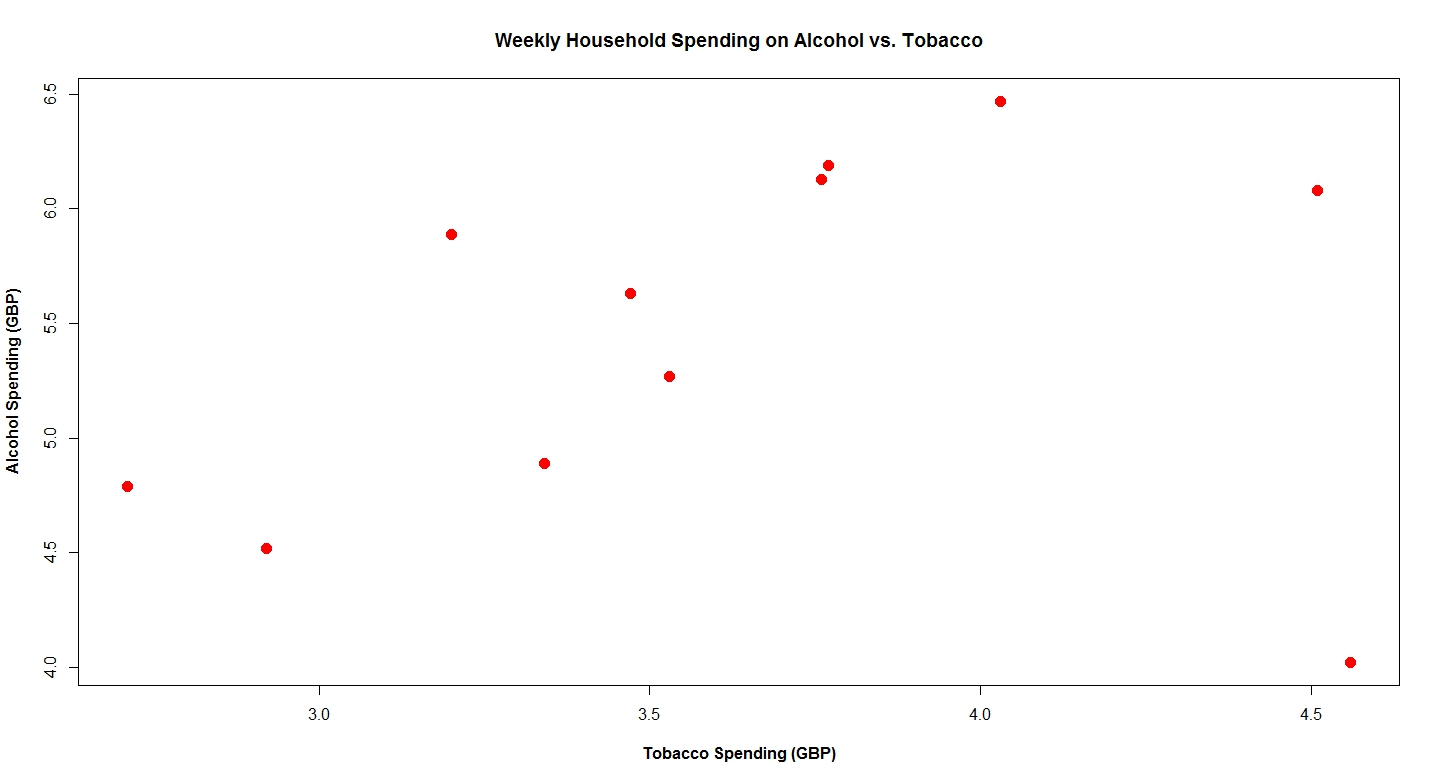
\includegraphics[width=1.3\linewidth]{alcotob}
		\caption{}
		\label{fig:alcotob}
	\end{figure}
	
	\begin{figure}
		\centering
		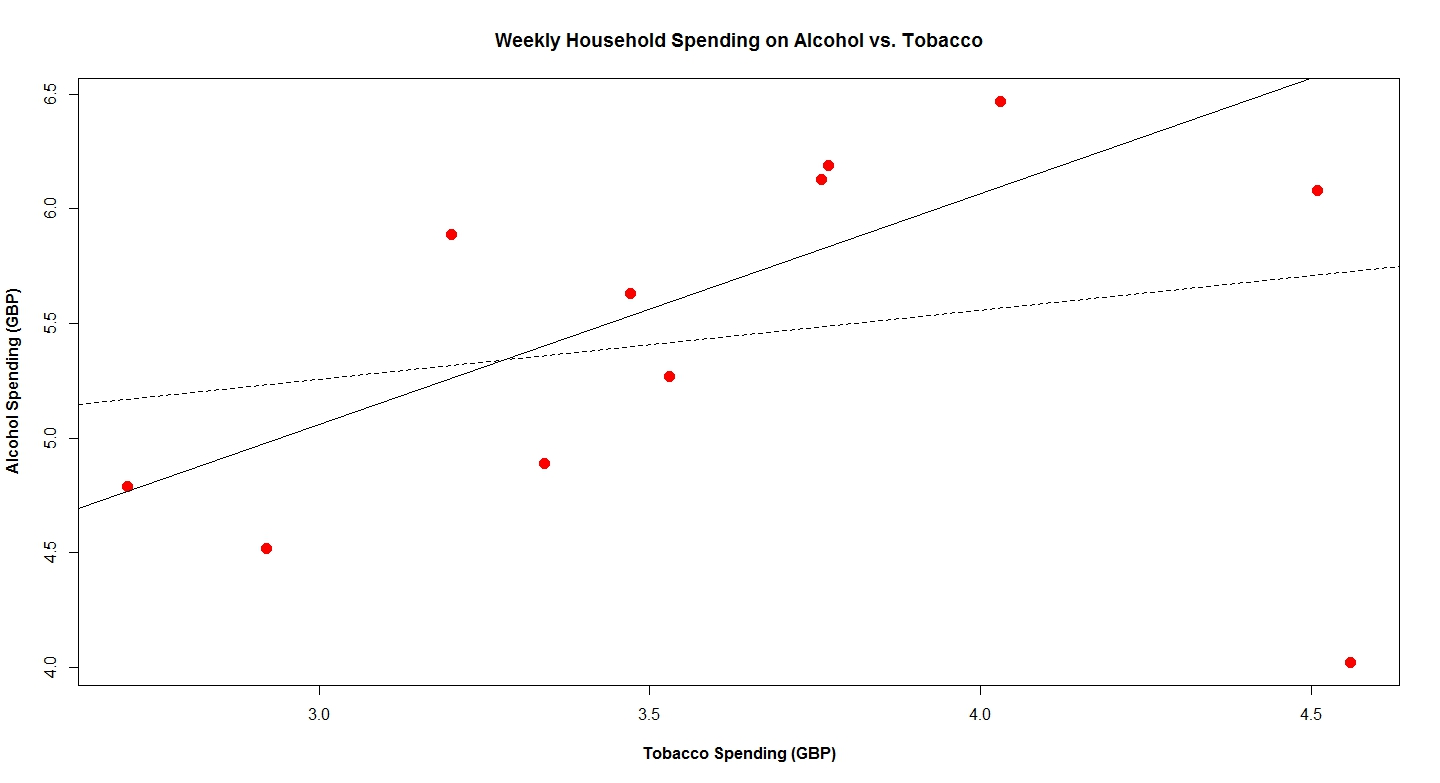
\includegraphics[width=1.3\linewidth]{alcotob2}
		\caption{}
		\label{fig:alcotob}
	\end{figure}
	\bigskip	
	\begin{framed}	
		\textbf{All Observations}	
		\begin{verbatim}
		> summary(fit1)
		
		Call:
		lm(formula = Alcohol ~ Tobacco, data = alctob)
		
		Residuals:
		Min      1Q  Median      3Q     Max 
		-1.7080 -0.4245  0.2311  0.6081  0.9020 
		
		Coefficients:
		Estimate Std. Error t value Pr(>|t|)  
		(Intercept)   4.3512     1.6067   2.708   0.0241 *
		Tobacco       0.3019     0.4388   0.688   0.5087  
		---
		Signif. codes:  0 ‘***’ 0.001 ‘**’ 0.01 ‘*’ 0.05 ‘.’ 0.1 ‘ ’ 1
		
		Residual standard error: 0.8196 on 9 degrees of freedom
		Multiple R-squared:  0.04998,   Adjusted R-squared:  -0.05557 
		F-statistic: 0.4735 on 1 and 9 DF,  p-value: 0.5087
		\end{verbatim}
	\end{framed}
	
	\begin{framed}
		\textbf{Outlier Removed	}
		\begin{verbatim}
		
		> summary(fit2)
		
		Call:
		lm(formula = Alcohol ~ Tobacco, data = alctobwo)
		
		Residuals:
		Min       1Q   Median       3Q      Max 
		-0.51092 -0.42434  0.06056  0.34406  0.62991 
		
		Coefficients:
		Estimate Std. Error t value Pr(>|t|)   
		(Intercept)   2.0412     1.0014   2.038  0.07586 . 
		Tobacco       1.0059     0.2813   3.576  0.00723 **
		---
		Signif. codes:  0 ‘***’ 0.001 ‘**’ 0.01 ‘*’ 0.05 ‘.’ 0.1 ‘ ’ 1
		
		Residual standard error: 0.446 on 8 degrees of freedom
		Multiple R-squared:  0.6151,    Adjusted R-squared:  0.567 
		F-statistic: 12.78 on 1 and 8 DF,  p-value: 0.007234
		
		\end{verbatim}
	\end{framed}
	
	\bigskip
	\subsection*{Outliers}
	
	
	
	
	The conservative outlier test that we talked about in class uses the
	Bonferonni inequality to calculate the p-values we associate with the
	Student's-t test. 
	
	In \texttt{R}, we can use the \texttt{outlierTest} command to perform this
	test on our model. Remember that when we test for influence, we are testing
	the effect of an observation on model coefficients. 
	
	Therefore we need to
	give the outlierTest command a linear model as its input.
	\begin{framed}
		\begin{verbatim}
		> # Assessing Outliers
		> # syntax: outlierTest(fit) 
		> # Bonferonni p-value for most extreme obs
		>
		> outlierTest(fit1)
		rstudent  unadjusted p-value Bonferonni p
		N. Ireland -4.732091           0.0014789     0.016268
		> 
		\end{verbatim}
	\end{framed}
	\noindent We can also use \texttt{R} to calculate Cook's distance. 
	%Remember that generally we label any observation with Cook's distance greater than 1 as influential.
	\begin{framed}
		\begin{verbatim}
		> cooks.distance(fit1)
		North           Yorkshire       Northeast     East Midlands 
		0.114101051     0.036517838     0.043728951   0.023600304 
		West Midlands   East Anglia     Southeast     Southwest 
		0.004740759     0.147326647     0.046646563   0.077488350 
		Wales           Scotland        N. Ireland 
		0.001821694     0.068921892     1.747233521 
		\end{verbatim}
	\end{framed}
	
	Finally, one of the easier ways to evaluate our residuals and look for
	for influential points is through plots. 
	
	\begin{framed}
		\begin{verbatim}
		#qq plot for studentized resid 
		qqPlot(fit1, main="QQ Plot",pch=18, lim=c(-3,2)) 
		
		# leverage plots
		leveragePlots(fit1) 
		\end{verbatim}
	\end{framed}
	
	\begin{figure}
		\centering
		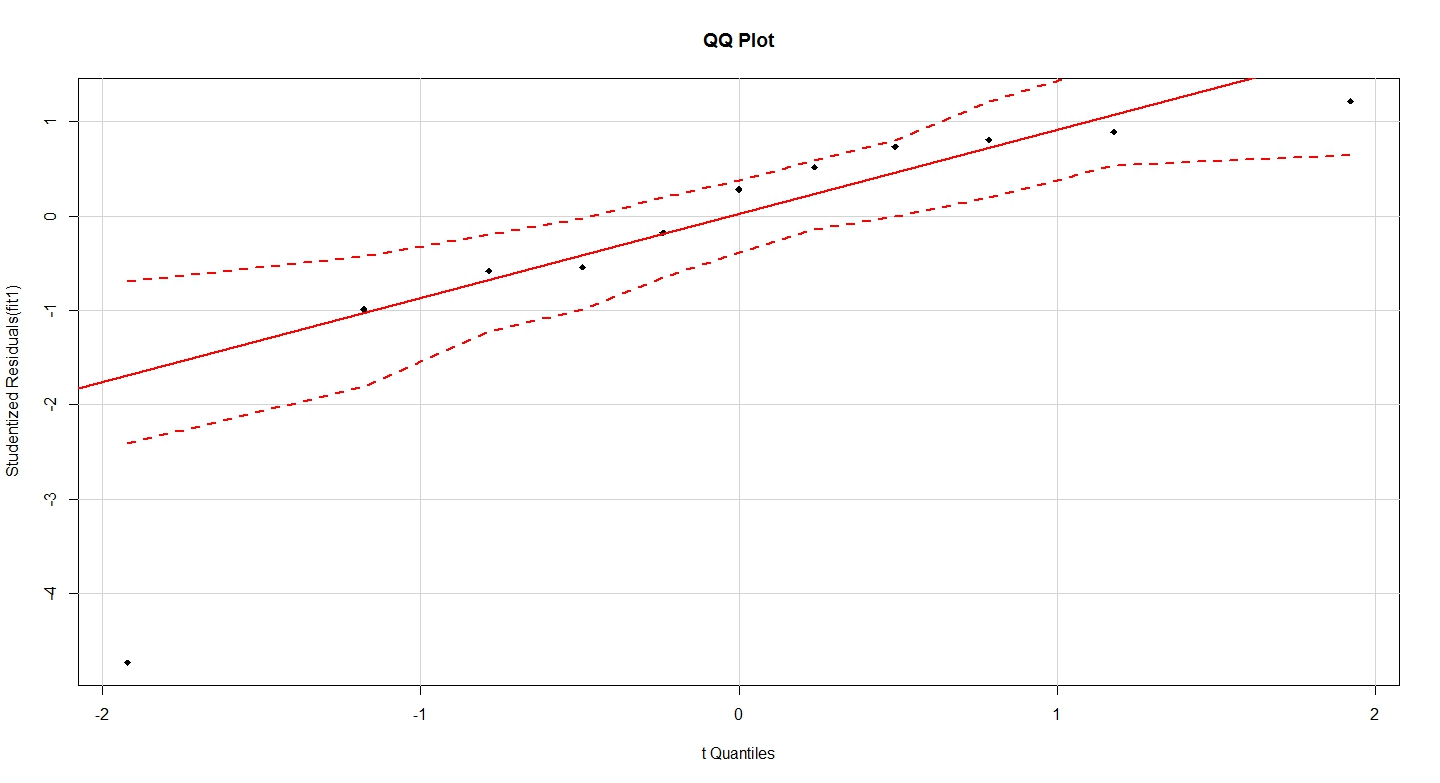
\includegraphics[width=1.2\linewidth]{alcotob3}
		%\caption{}
		%\label{fig:alcotob3}
	\end{figure}
	
	
	\begin{figure}
		\centering
		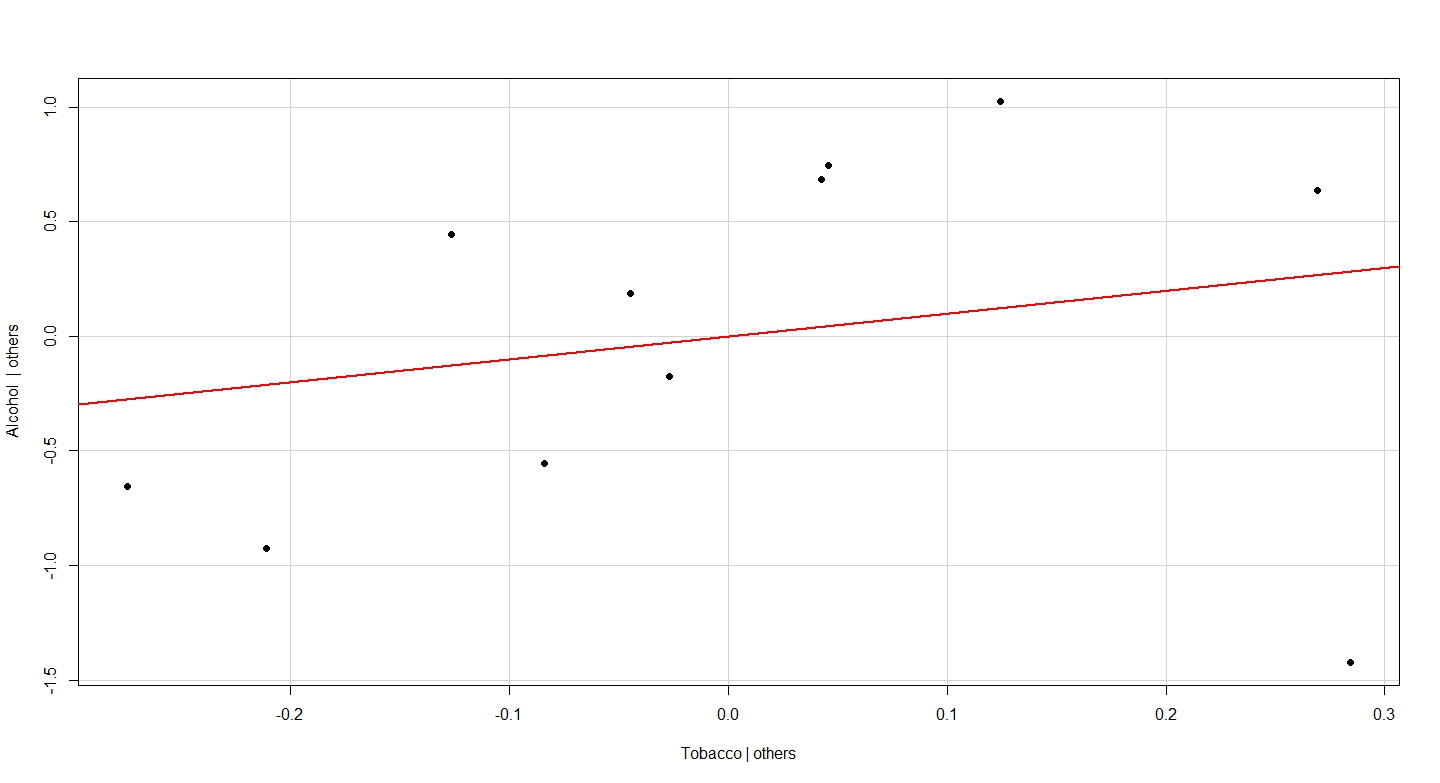
\includegraphics[width=1.2\linewidth]{alcotob4}
		%\caption{}
		%\label{fig:alcotob3}
	\end{figure}
	
	
	% In \texttt{R}, the \texttt{plot} command takes a
	% special form when you pass it an \texttt{lm} object (see ?plot.lm for all of the
	% details). 
	
	
	
	
	\bigskip
	\begin{framed}
		\begin{verbatim}
		Influential Observations
		# Influential Observations
		# added variable plots 
		avPlots(fit1)
		
		
		# Cook's D plot
		# identify D values > 4/(n-k-1) 
		cutoff <- 4/((nrow(mtcars)-length(fit1$coefficients)-2)) 
		plot(fit, which=4, cook.levels=cutoff)
		\end{verbatim}
	\end{framed}
	\begin{figure}
		\centering
		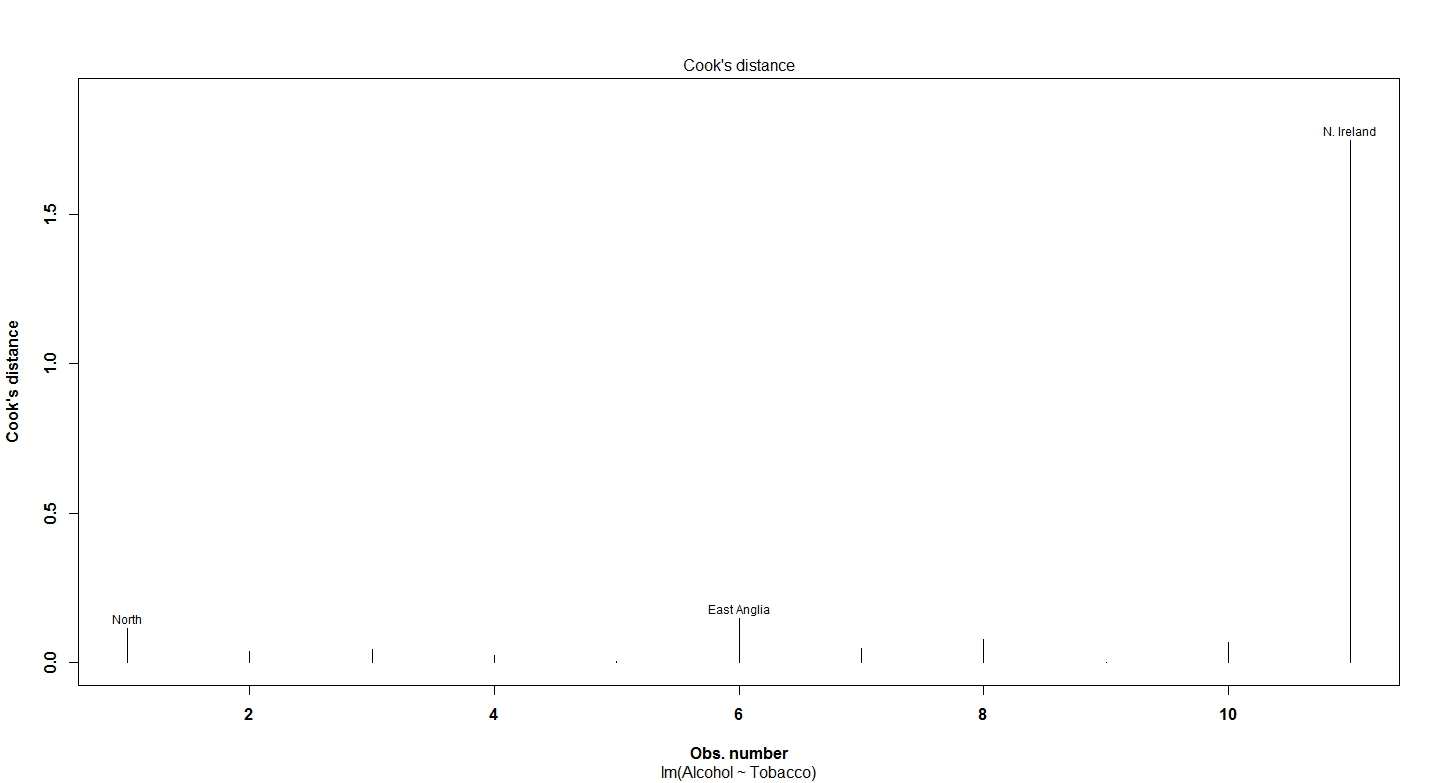
\includegraphics[width=0.7\linewidth]{alcotob6}
		\caption{}
		\label{fig:alcotob6}
	\end{figure}
	
	\bigskip
	\begin{framed}
		\begin{verbatim}
		# Influence Plot 
		influencePlot(fit1,	id.method="identify", 
		main="Influence Plot", 
		col="red"
		sub="Circle size is proportial to Cook's Distance" )
		
		\end{verbatim}
	\end{framed}
	\subsection*{Non-normality}
	
	\begin{framed}
		\begin{verbatim}
		
		# Normality of Residuals
		# qq plot for studentized resid
		qqPlot(fit1, main="QQ Plot")
		\end{verbatim}
	\end{framed}
	
	\begin{framed}
		\begin{verbatim}
		# distribution of studentized residuals
		library(MASS)
		sresid <- studres(fit) 
		hist(sresid, freq=FALSE, 
		main="Distribution of Studentized Residuals")
		xfit<-seq(min(sresid),max(sresid),length=40) 
		yfit<-dnorm(xfit) 
		lines(xfit, yfit)
		\end{verbatim}
	\end{framed}
	\subsection*{Non-constant Error Variance}
	\begin{framed}
		\begin{verbatim}	
		
		
		# Evaluate homoscedasticity
		# non-constant error variance test
		ncvTest(fit)
		# plot studentized residuals vs. fitted values 
		spreadLevelPlot(fit)
		\end{verbatim}
	\end{framed}
	\subsection*{Multi-collinearity}
	\begin{framed}
		\begin{verbatim}
		
		# Evaluate Collinearity
		vif(fit) # variance inflation factors 
		sqrt(vif(fit)) > 2 # problem?
		\end{verbatim}
	\end{framed}
	%================================================================= %
	\subsection{Nonlinearity}
	\begin{framed}
		\begin{verbatim}	
		
		# Evaluate Nonlinearity
		# component + residual plot 
		crPlots(fit)
		# Ceres plots 
		ceresPlots(fit)
		
		# Non-independence of Errors
		# Test for Autocorrelated Errors
		durbinWatsonTest(fit)
		\end{verbatim}
	\end{framed}
	\subsection{Additional Diagnostic Help}
	The gvlma( ) function in the gvlma package, performs a global validation of linear model assumptions as well separate evaluations of skewness, kurtosis, and heteroscedasticity.
	\begin{framed}
		\begin{verbatim}
		# Global test of model assumptions
		library(gvlma)
		gvmodel <- gvlma(fit) 
		summary(gvmodel)
		\end{verbatim}
	\end{framed}
	% \subsection{Going Further}
	% If you would like to delve deeper into regression diagnostics, two books written by John Fox can help: Applied regression analysis and generalized linear models (2nd ed) and An R and S-Plus companion to applied regression.
	
\end{document}
